\chapter{Fundamental Geometry}

\section{Fundamental 01 - Segments}

A \textbf{Segment} (đoạn thẳng) $\overline{AB}$ has finite length.

A \textbf{Line} (đường thẳng) $\overleftrightarrow{AB}$ extends out indefinitely in both directions.

A \textbf{Ray} (tia) $\overrightarrow{AB}$ only extends in one direction

A \textbf{Plane} (mặt phẳng) $ABC$. You cannot choose collinear points to notate a plane because there is an infinite number of planes that can go through that line and can be rotated.

The \textbf{intersection} of two lines is a \textbf{point} (một điểm).

The \textbf{intersection} of two planes is a line.

\textbf{Collinear points} are points that lie on the same straight line.

\textbf{Coplanar points} are points that all lie on the same plane. Any two points are always coplanar, and any three points are always coplanar, even if they are collinear (on the same line). However, four or more points are coplanar only if they all lie on the same plane

\textbf{Opposite rays} (tia đối) are two rays that share the same endpoint and extend in exactly opposite directions. Together, they form a straight line.

\begin{figure}[ht]
  \centering
  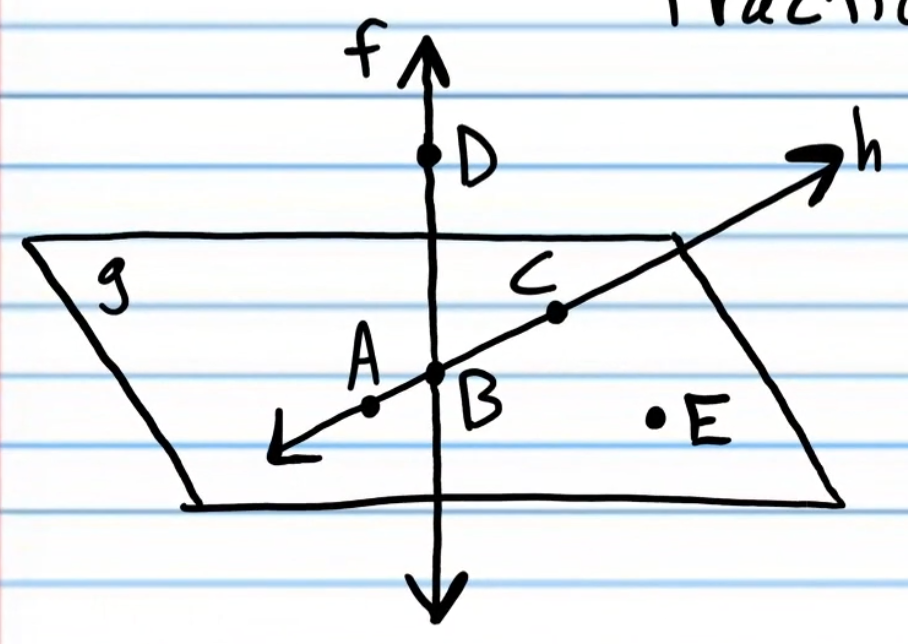
\includegraphics[width=0.5\textwidth]{0201.png}
  \caption{Bài tập}
\end{figure}

Name three collinear points on the figure above: A, B and C

Name four coplanar points: A, B, C and E

\vspace{10 mm}

\begin{figure}[ht]
  \centering
  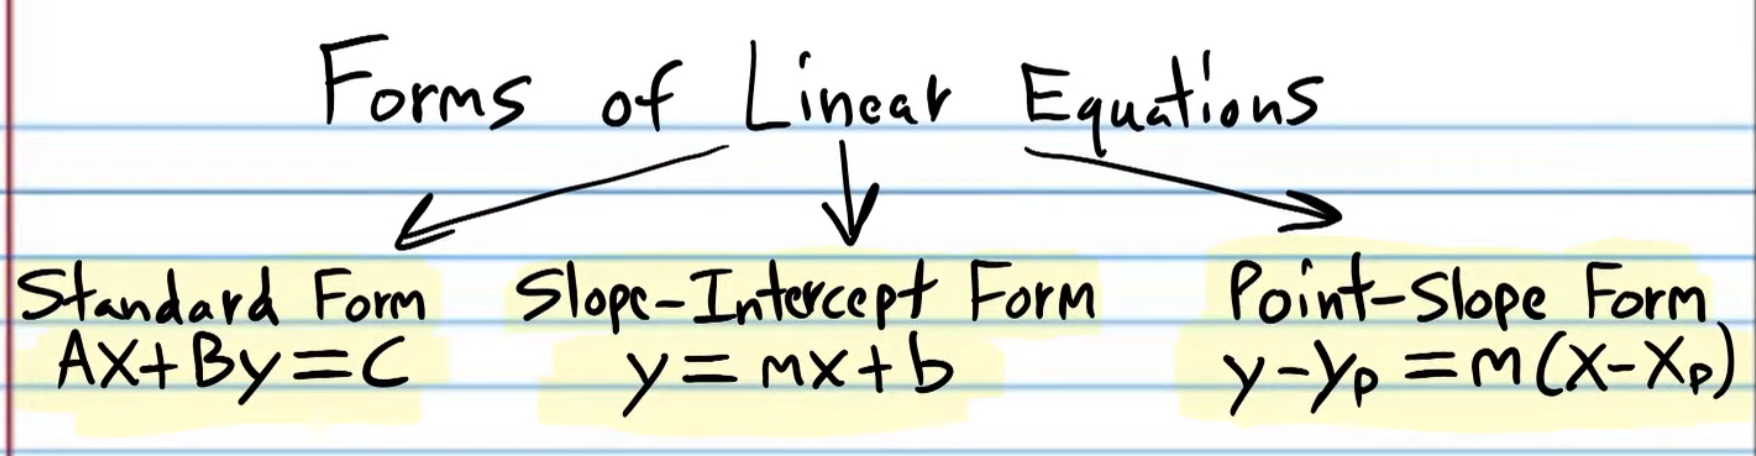
\includegraphics[width=0.6\textwidth]{0202.png}
  \caption{Bài tập}
\end{figure}

01: What is another name for FEH?

\textbf{A}: You can \textbf{NOT} name that plane IQK or FLE because those are collinear points.Any plane that goes through those two lines and can be rotated around is a possible plane. You have to choose three points that are not collinear.

\begin{figure}[h!]
  \centering
  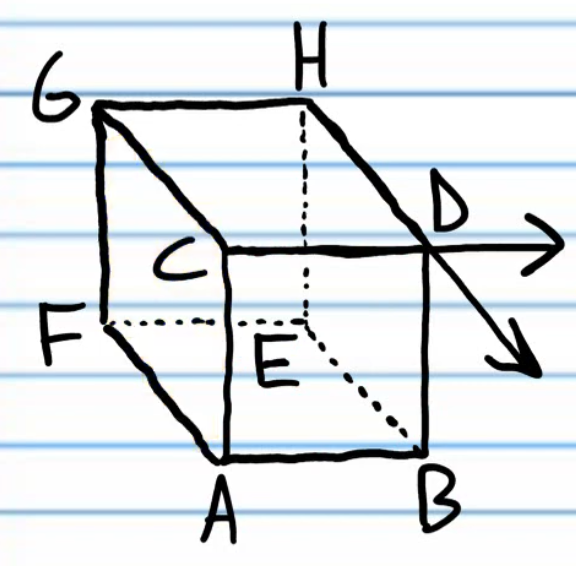
\includegraphics[width=0.6\textwidth]{0203.png}
  \caption{Bài tập}
\end{figure}

\textbf{Note}: These are planes with Finite length which means that their intersection will be segments, not lines.

01: Name three planes that intersect at B.

CAB, FEB and HDB

$\bigstar$ 02: Are F, E and A coplanar?

Any three points are always coplanar. There is at least one plane. Nếu 3 điểm colliner thì có infinite planes (you can rotate the planes).

$\bigstar$ 03: Are A and G collinear?

We don't even need to look at the picture. Any two points are collinear.

$\bigstar$ 04: Are A and H coplanar?

You can make an infinite number of planes that goes through any two points.

% \par creates a paragraph break
% \noindent prevents indentation of the current paragraph (the dot line in this case)
\par\noindent\dotfill

\textbf{Postulate} (also called an axiom): A statement that is accepted without an explanation or proof.

Theorem: A statement that requires an explanation or proof that uses definitions, postulates, other theorems, logic, etc.

\vspace{1 cm}

\centerline{\textbf{\huge Segments}}

\vspace{0.2 cm}

If $\overline{AB}$ is a segment, then AB is defined as its length (without the overline on top).

\hl{Congruence}: Having the same size and shape (notated by $\cong$). For example two triangles can be congruent.

If two segments are to be congruent, then they must have the same lengths (không cần phải cùng hướng hay song song gì cả).

Example: If $\overline{AB} \cong \overline{CD}$, then AB=CD.

\hl{The Segment Addition Postulate}: If A, B, and C are collinear, and B is between A and C, then $AB + BC = AC$.

\begin{figure}[h]
  \centering
  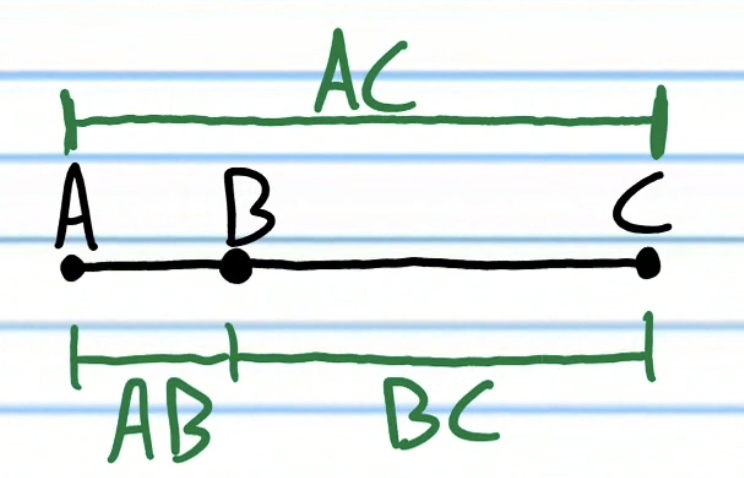
\includegraphics[width=0.4\textwidth]{0204.png}
  \caption{The Segment Addition Postulate}
\end{figure}

\hl{Midpoint of a Segment}: A point (e.g. M below) that is in the middle or center of a segment, dividing it into two congruent segments.

\begin{figure}[h]
  \centering
  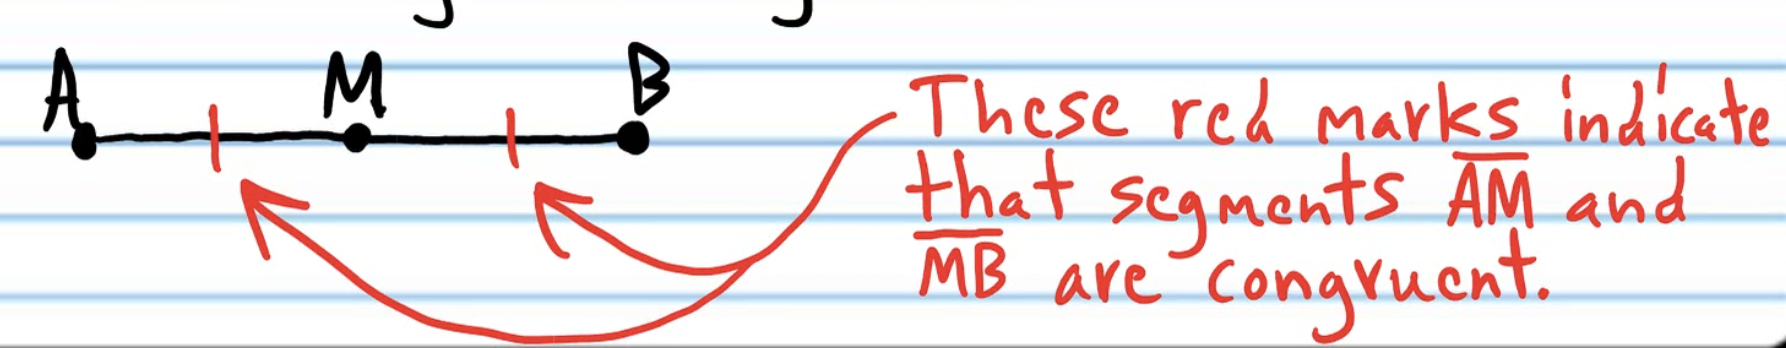
\includegraphics[width=0.7\textwidth]{0205.png}
  \caption{Midpoint of a Segment}
\end{figure}

\hl{Bisect}: (verb) To divide into two \textbf{equal} parts.

\hl{Segment Bisector}: A point, ray, line, segment or plane that divides a segment into two congruent segments by intersecting at its midpoint.

\begin{figure}[htb!]
  \centering
  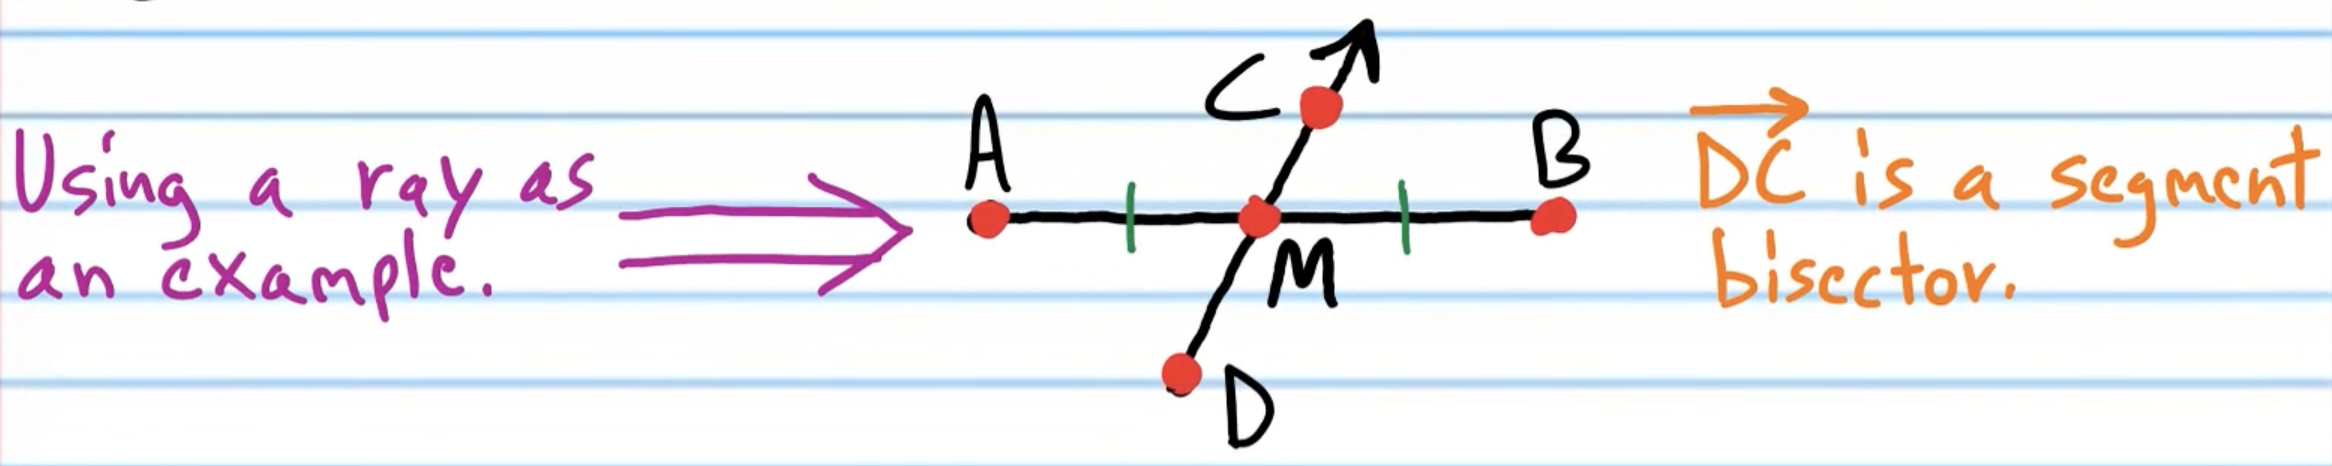
\includegraphics[width=0.7\textwidth]{0206.png}
  \caption{Segment Bisector}
\end{figure}

\section{Fundamental 02 - Angles}

\hl{Angle}: Two \textbf{rays} with a common \textbf{endpoint} that help to indicate a measure of rotation.

\begin{figure}[htb!]
  \centering
  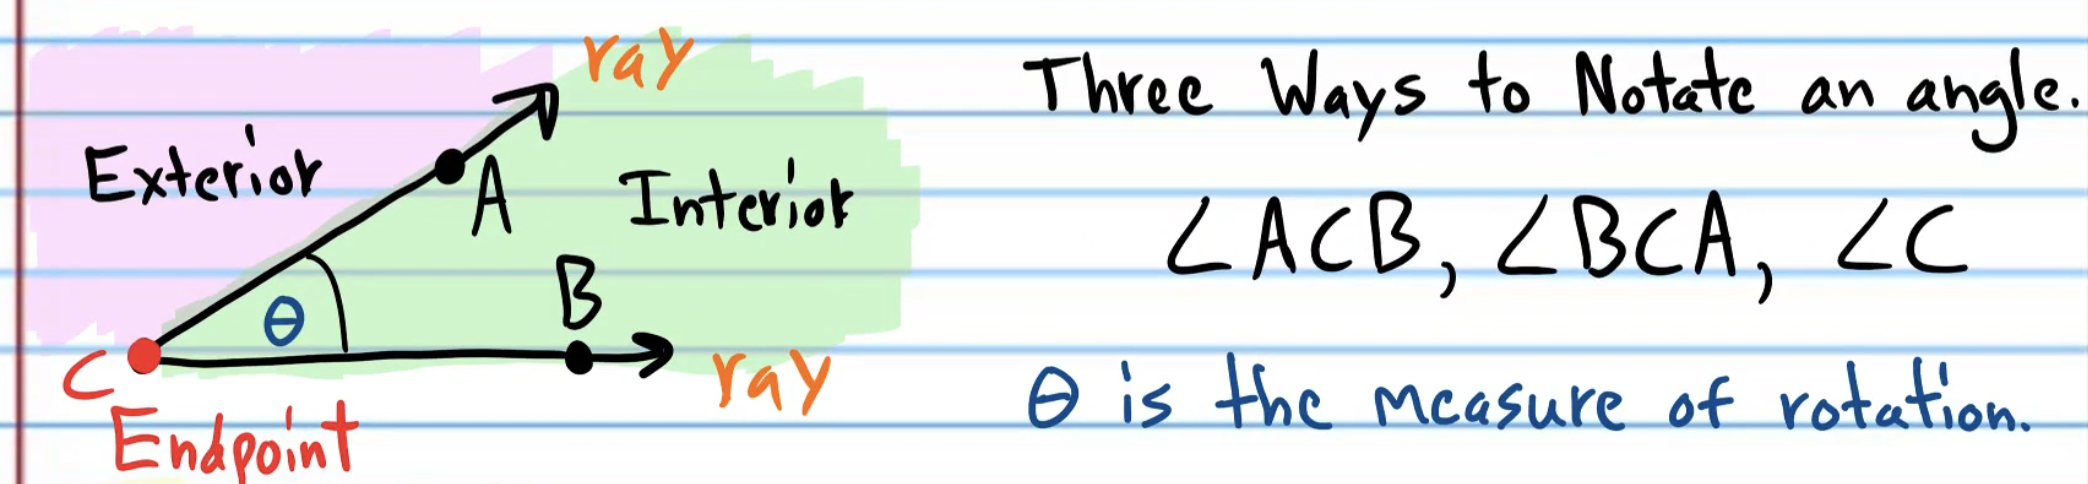
\includegraphics[width=0.7\textwidth]{0301.png}
  \caption{An Angle}
\end{figure}

\hl{Angle Vertex}: The common \textbf{endpoint} of the two \textbf{rays}.

\hl{Angle Sides}: The two \textbf{rays}.

$\angle ABC$ refer to the concept of the angle. You can write a letter m in front like $m\angle ABC$ to represents the measure of the angle (which is just a number). Or you can also use a Greek letter (e.g. $\theta$).

\vspace{1 cm}

\centerline{\textbf{\huge Classifying Angles}}

\vspace{0.2 cm}

\hl{Right Angle} góc vuông $90^{\circ}$

\hl{Acute angle} (Góc nhọn): $0^{\circ} < \Theta < 90^{\circ}$

\hl{Straight Angle} góc bẹt $180^{\circ}$

\hl{Obtuse angle} (Góc tù) $90^{\circ} < \Theta < 180^{\circ}$

\hl{Reflex angle} (Góc lõm) $180^{\circ} < \Theta < 360^{\circ}$

\hl{Full angle} $\Theta = 360^{\circ}$

\newpage

Angle Addition Postulate. Postulate is what we accept to be true without requiring any explanation.

\begin{figure}[htb!]
  \centering
  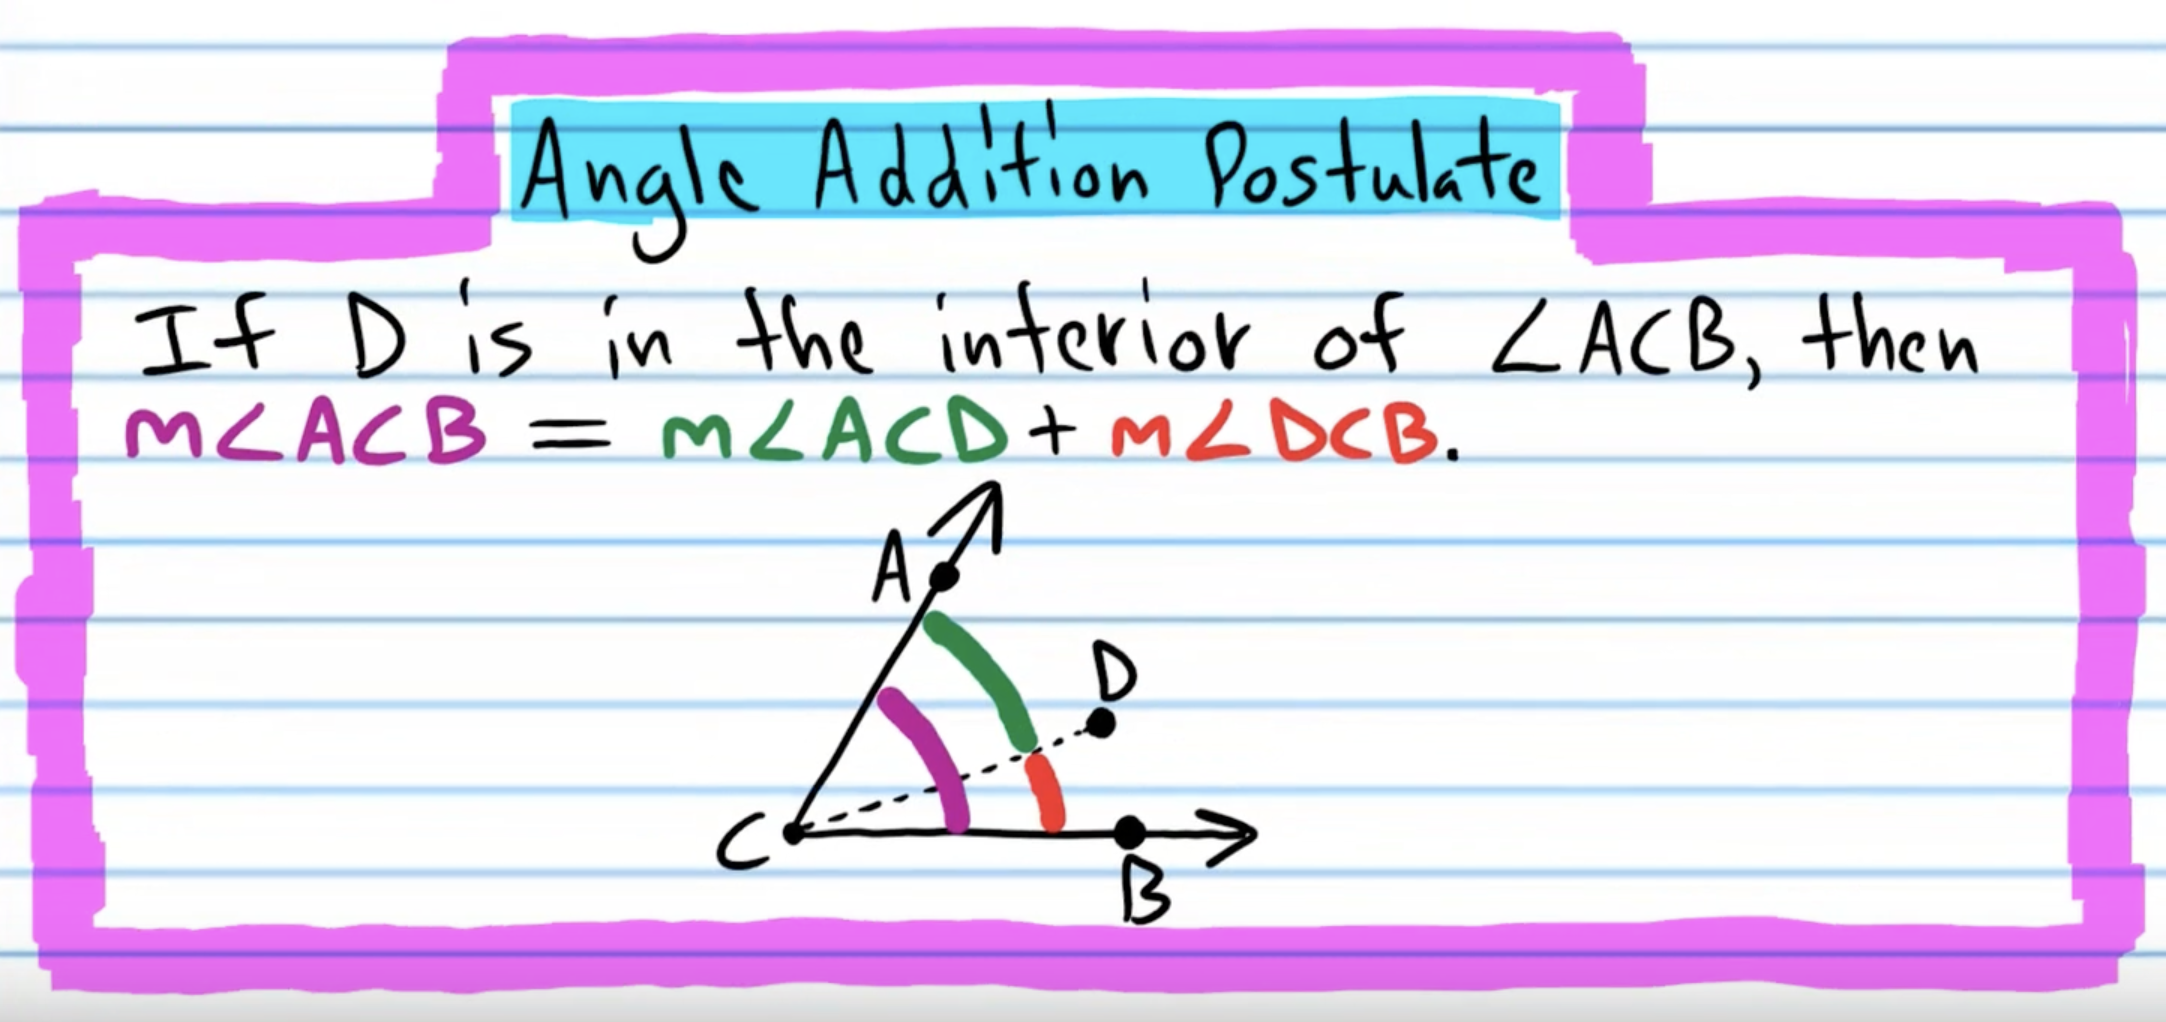
\includegraphics[width=0.7\textwidth]{0302.png}
  \caption{Angle Addition Postulate}
\end{figure}

If two angles are \textbf{congruent}, then their measures are equal. We write $\angle ABD \cong \angle DBC$ but $m\angle ABD = m\angle DBC$.

\hl{Angle Bisector}: A \textbf{ray} that divides an angle in half, such that the two resulting angles are congruent.

\vspace{0.9 cm}

\centerline{\textbf{\huge Angle Pairs}}

\vspace{0.2 cm}

\hl{Adjacent Angles}: Two angles that share a vertex and a side but have no common interior points.

\begin{figure}[htb!]
  \centering
  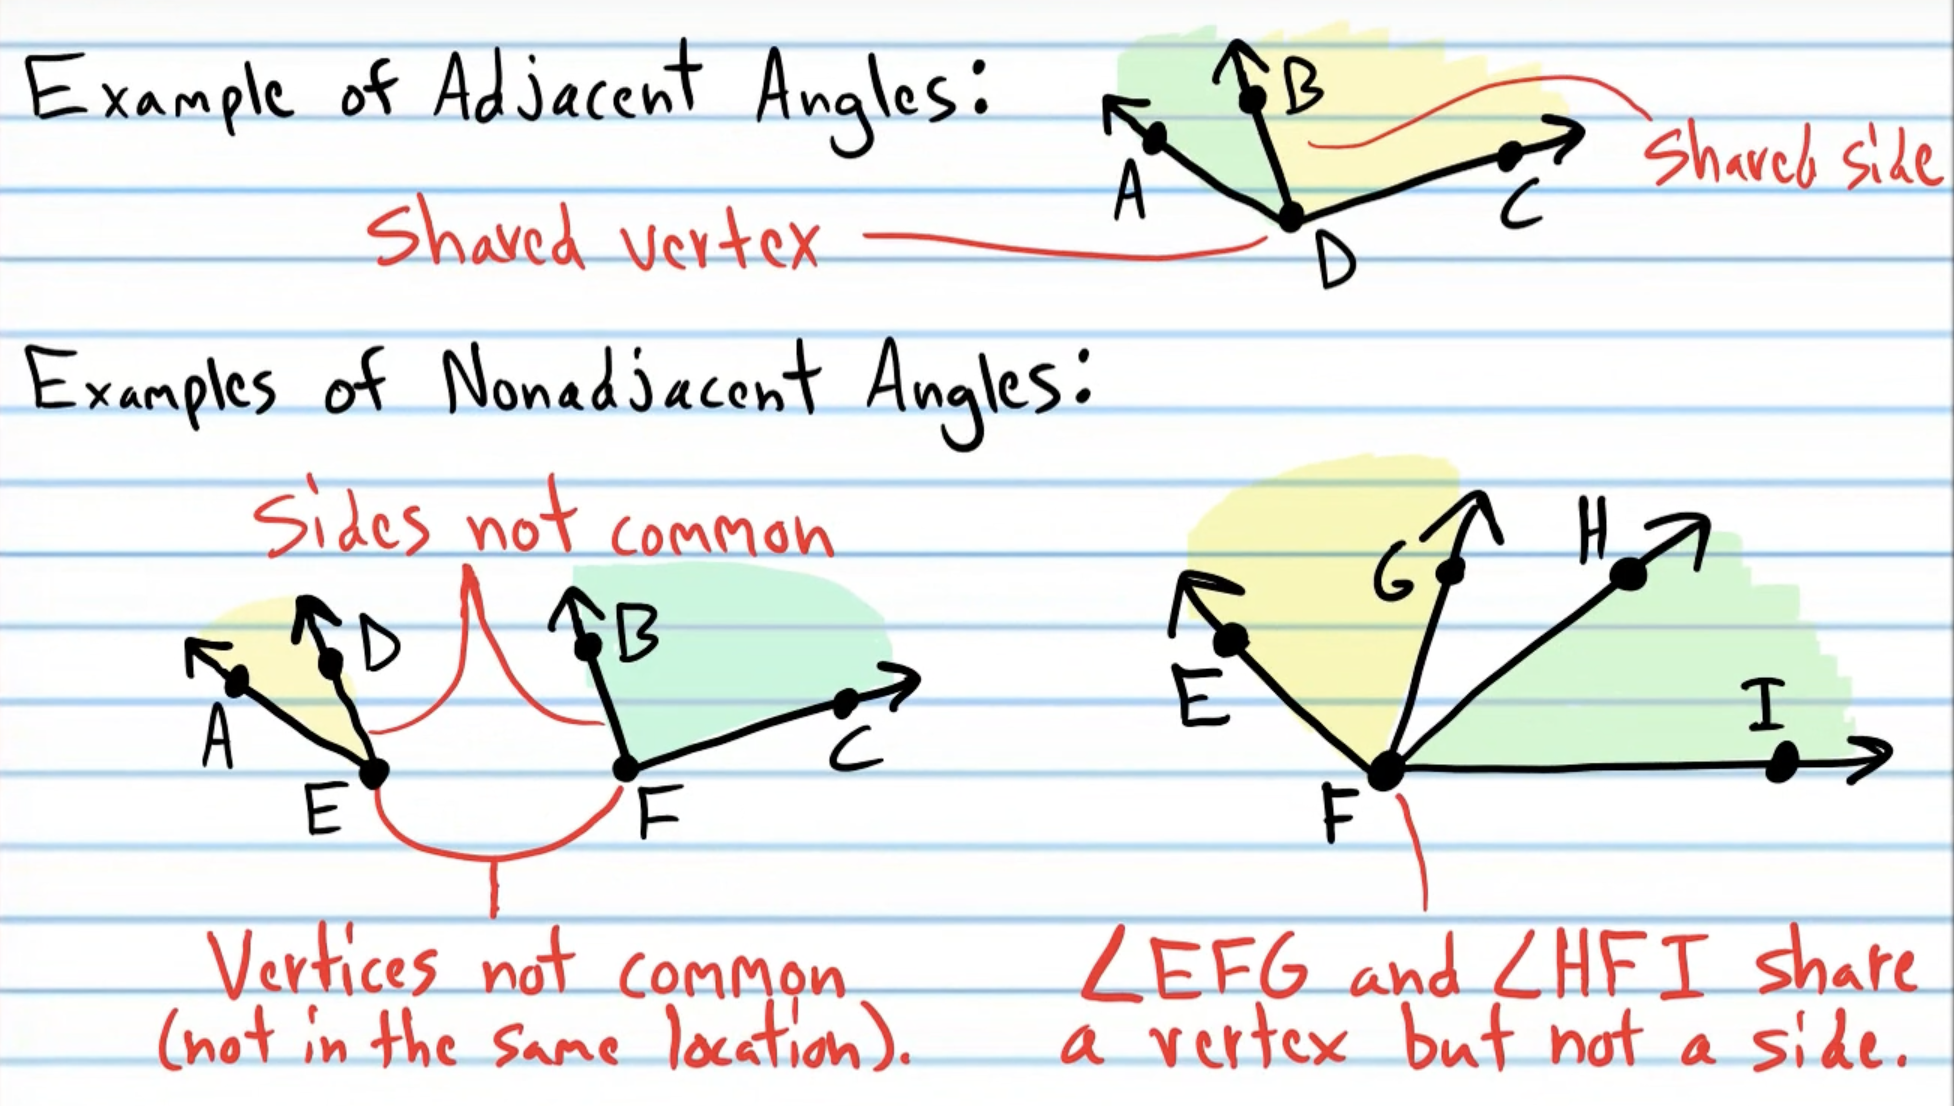
\includegraphics[width=0.9\textwidth]{0303.png}
  \caption{Adjacent Angles}
\end{figure}

\newpage

\hl{Complementary Angles}: Two angles whose measures add up to $90^{\circ}$.

\begin{figure}[htb!]
  \centering
  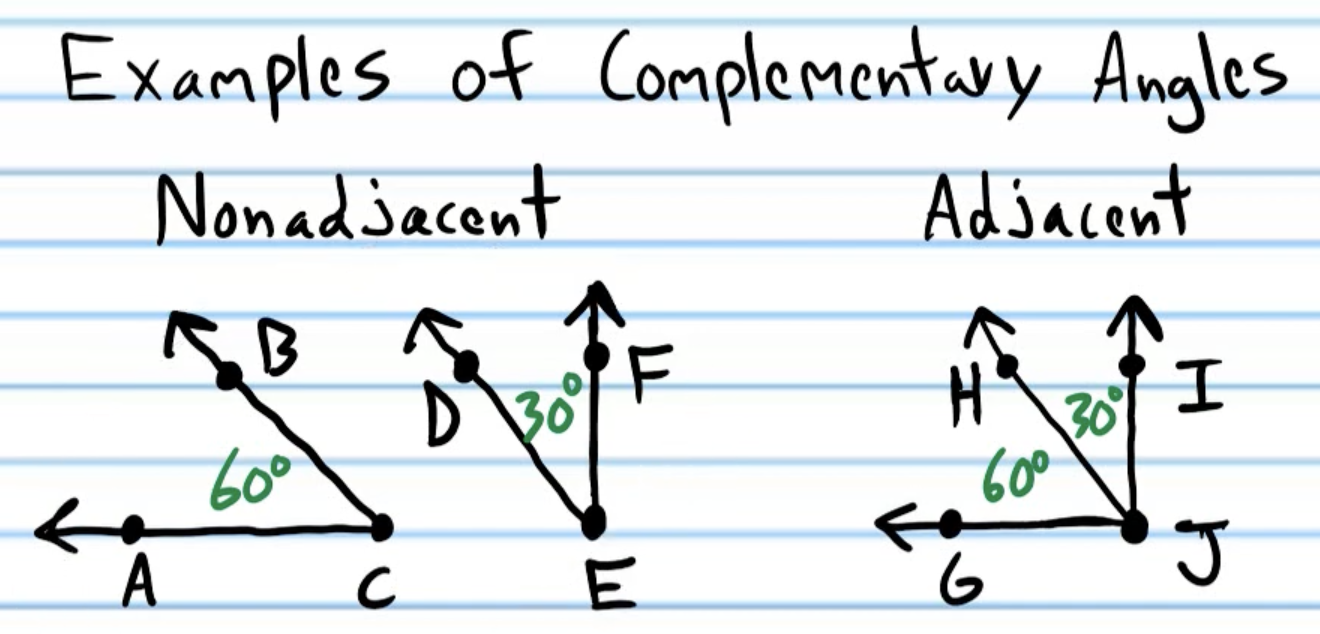
\includegraphics[width=0.7\textwidth]{0304.png}
  \caption{Complementary Angles}
\end{figure}

Compliment spelled with an \q{i} is a comment that expresses praise or approval of somebody. But Complement with an \q{e} means you make something better by adding something to it.

Remember the \q{c} in complement => Chín chục.

\vspace{10 mm}

\hl{Supplementary Angles}: Two angles whose measures add up to $180^{\circ}$.

\begin{figure}[htb!]
  \centering
  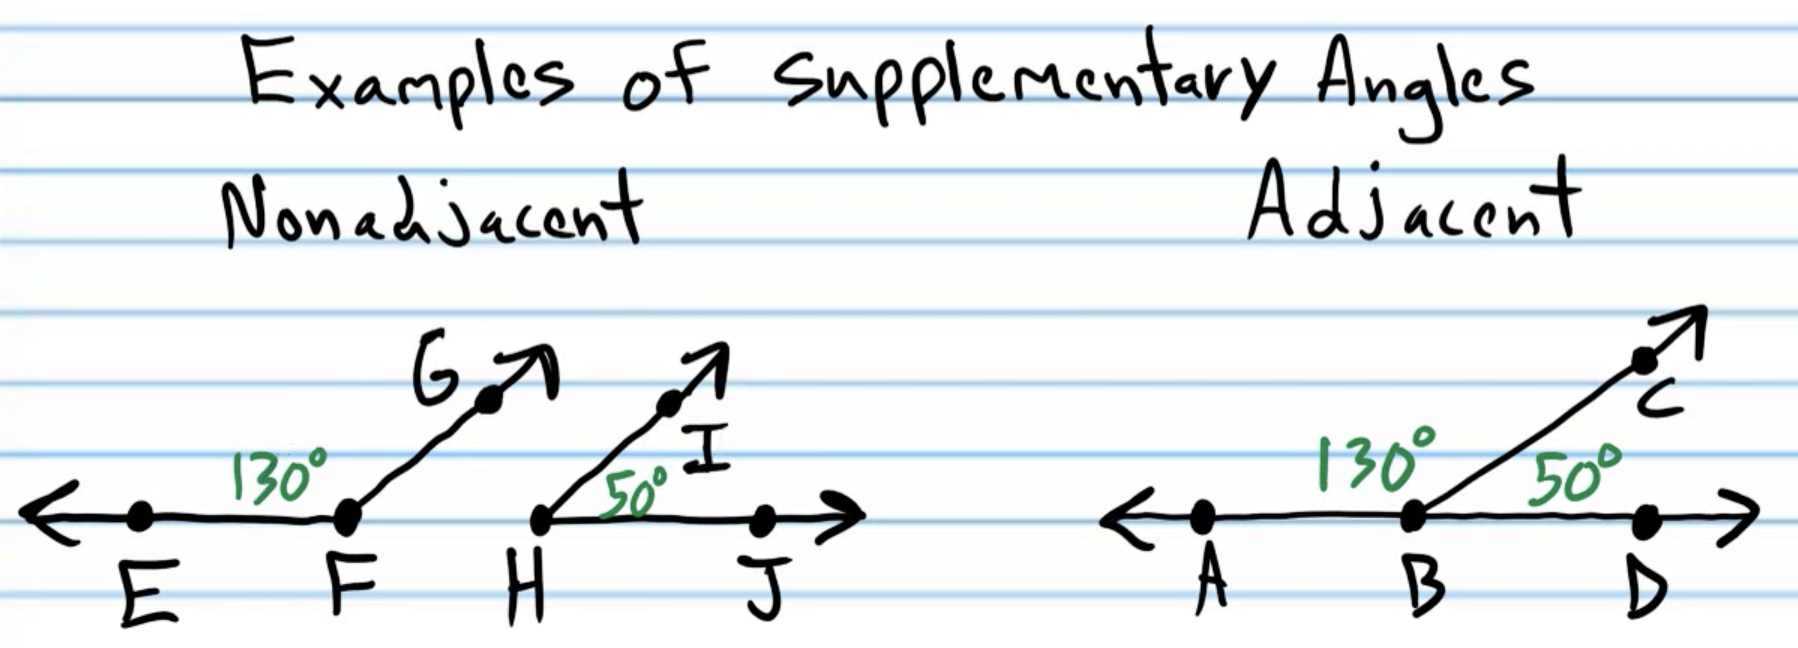
\includegraphics[width=0.7\textwidth]{0305.png}
  \caption{Supplementary Angles}
\end{figure}

\textbf{Bai tập 25}: If the measure of an angle is $40^{\circ}$ less than the measure of its supplement, what is the measure of the angle?

\vspace{0.2 cm}

\centerline{\textbf{\normalsize Answer}}

\vspace{0.2 cm}

Giải system of equation below bằng substitution:

\begin{equation*}
    \begin{cases}
      m\angle A + m\angle B = 180\\
      m\angle A = m\angle B -40
    \end{cases}\,.
\end{equation*}

\vspace{5 cm}

\hl{Linear Pair}: Two adjacent angles whose non-common sides are opposite rays.

\begin{figure}[htb!]
  \centering
  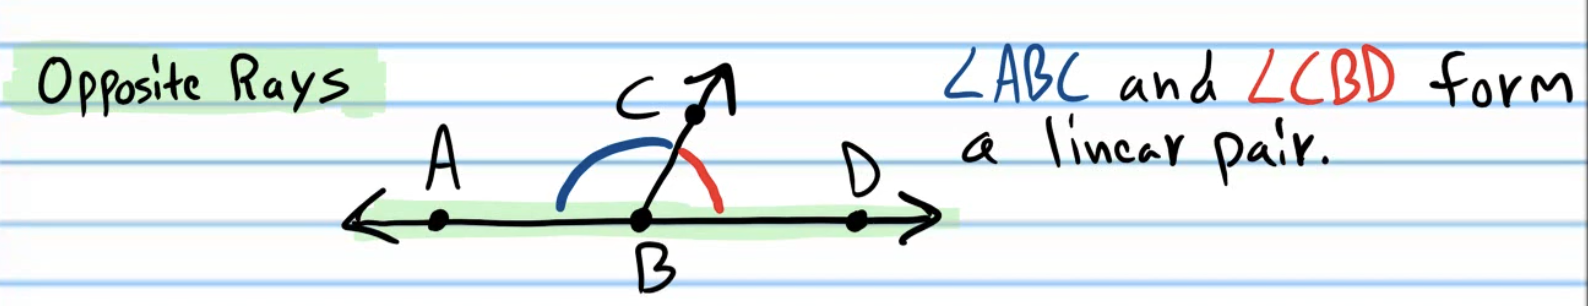
\includegraphics[width=0.8\textwidth]{0306.png}
  \caption{Linear Pair}
\end{figure}

% \colorbox{SkyBlue}{Linear Pair Postulate}: If two angles from a linear pair, they are supplementary.

\begin{tcolorbox}[colback=RoyalPurple!5!white,colframe=RoyalPurple!75!black]
  \colorbox{SkyBlue}{Linear Pair Postulate}: If two angles from a linear pair, they are supplementary.
\end{tcolorbox}

\vspace{1 cm}

\hl{Vertical Angles}: Two angles whose sides form two pairs of opposite rays. Or when two lines intersect.

\begin{figure}[htb!]
  \centering
  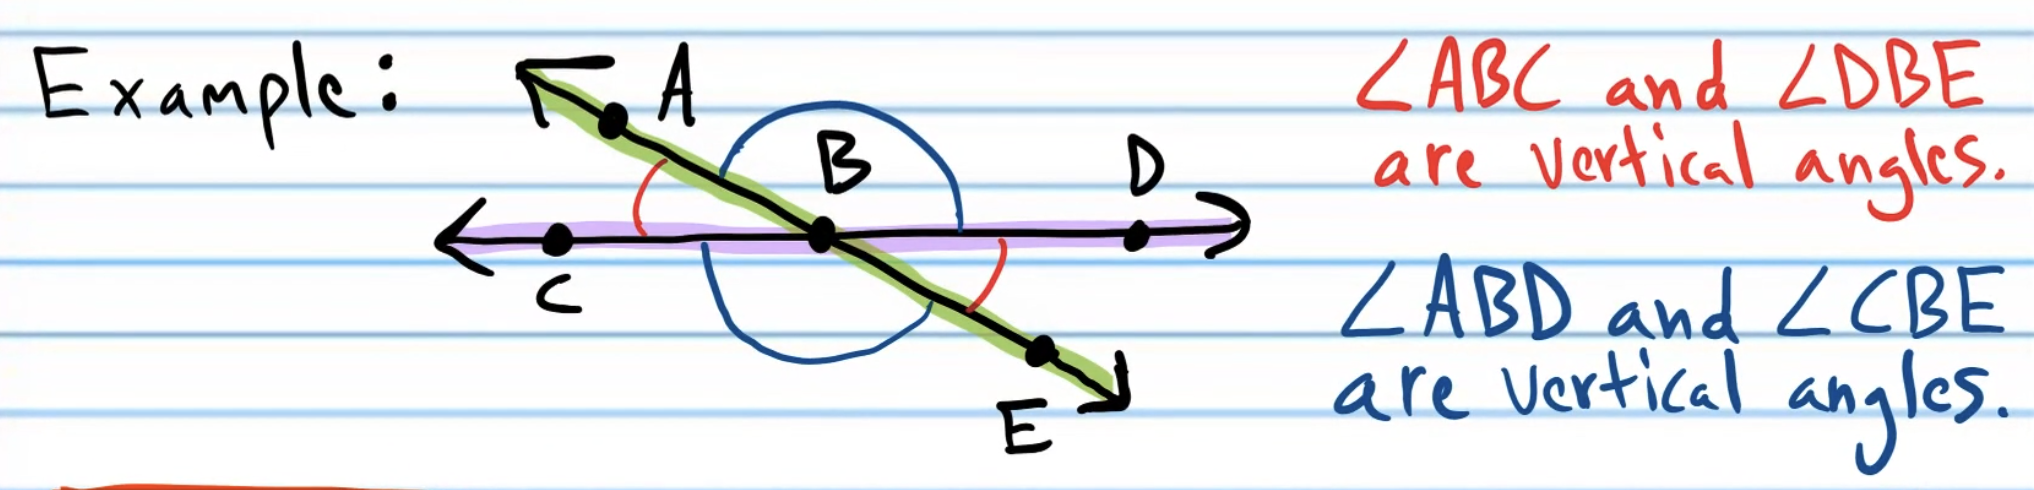
\includegraphics[width=0.8\textwidth]{0307.png}
  \caption{Vertical Angles}
\end{figure}

\begin{tcolorbox}[colback=red!5!white,colframe=red!75!black]
  \colorbox{Orange}{Vertical Angles Theorem}: Vertical angles are congruent.
\end{tcolorbox}

\section{Fundamental 03 - Polygons}

\hl{Polygon}: A closed plane figure whose sides are segments that intersects only at endpoints.

\begin{figure}[htb!]
  \centering
  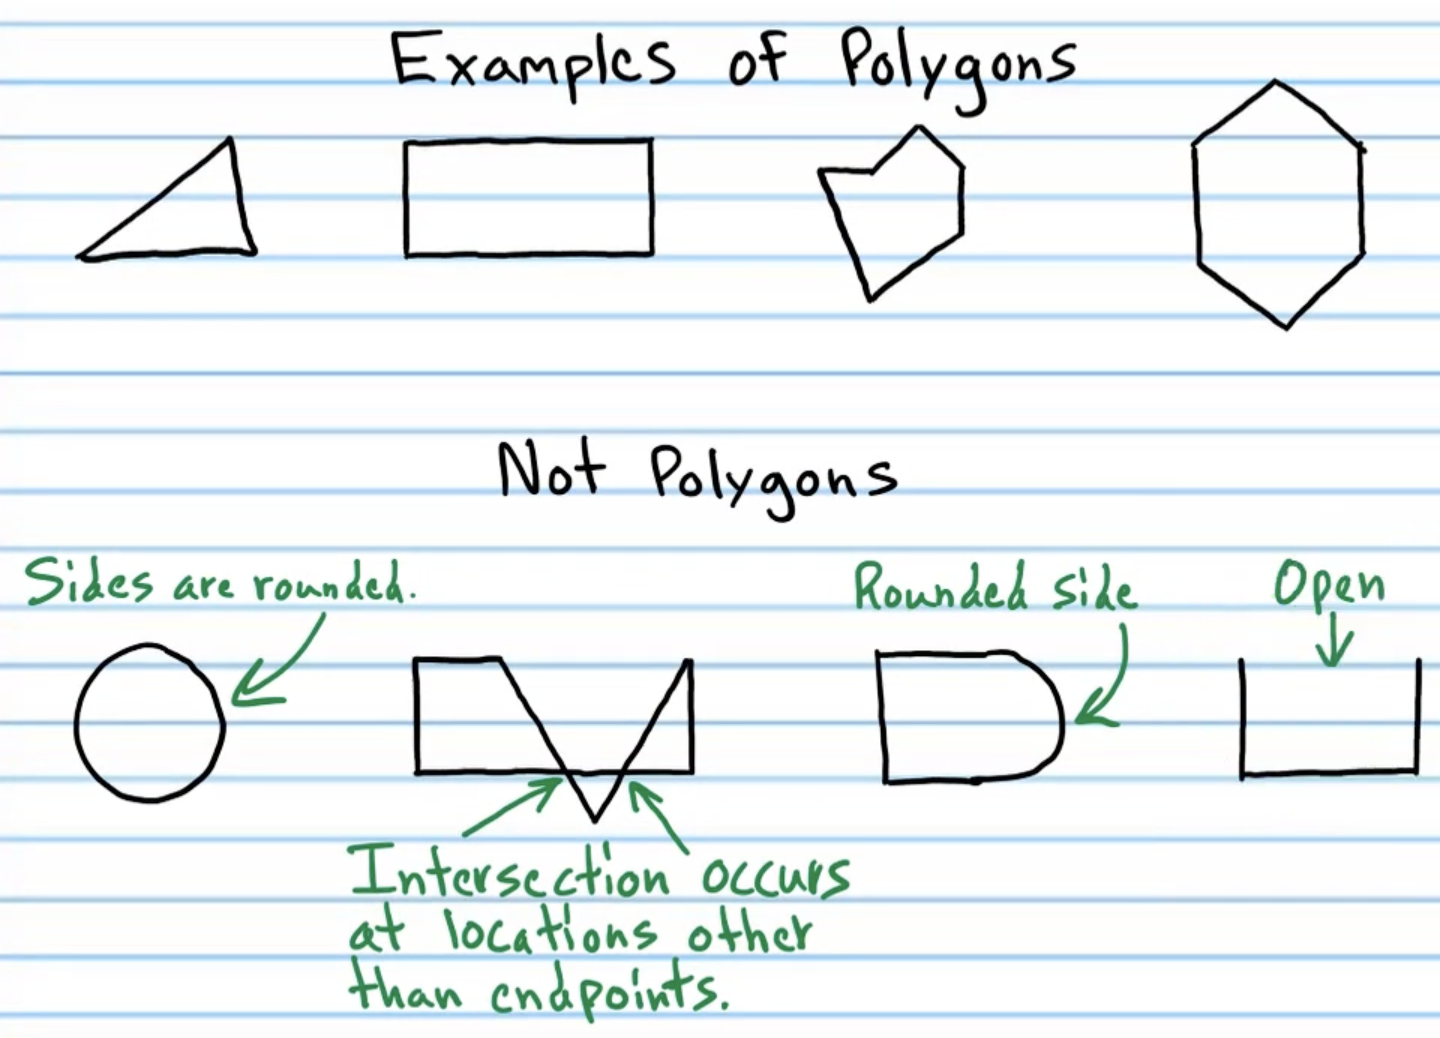
\includegraphics[width=0.7\textwidth]{0401.png}
  \caption{Polygons}
\end{figure}

Parts of a Polygon.

\begin{figure}[htb!]
  \centering
  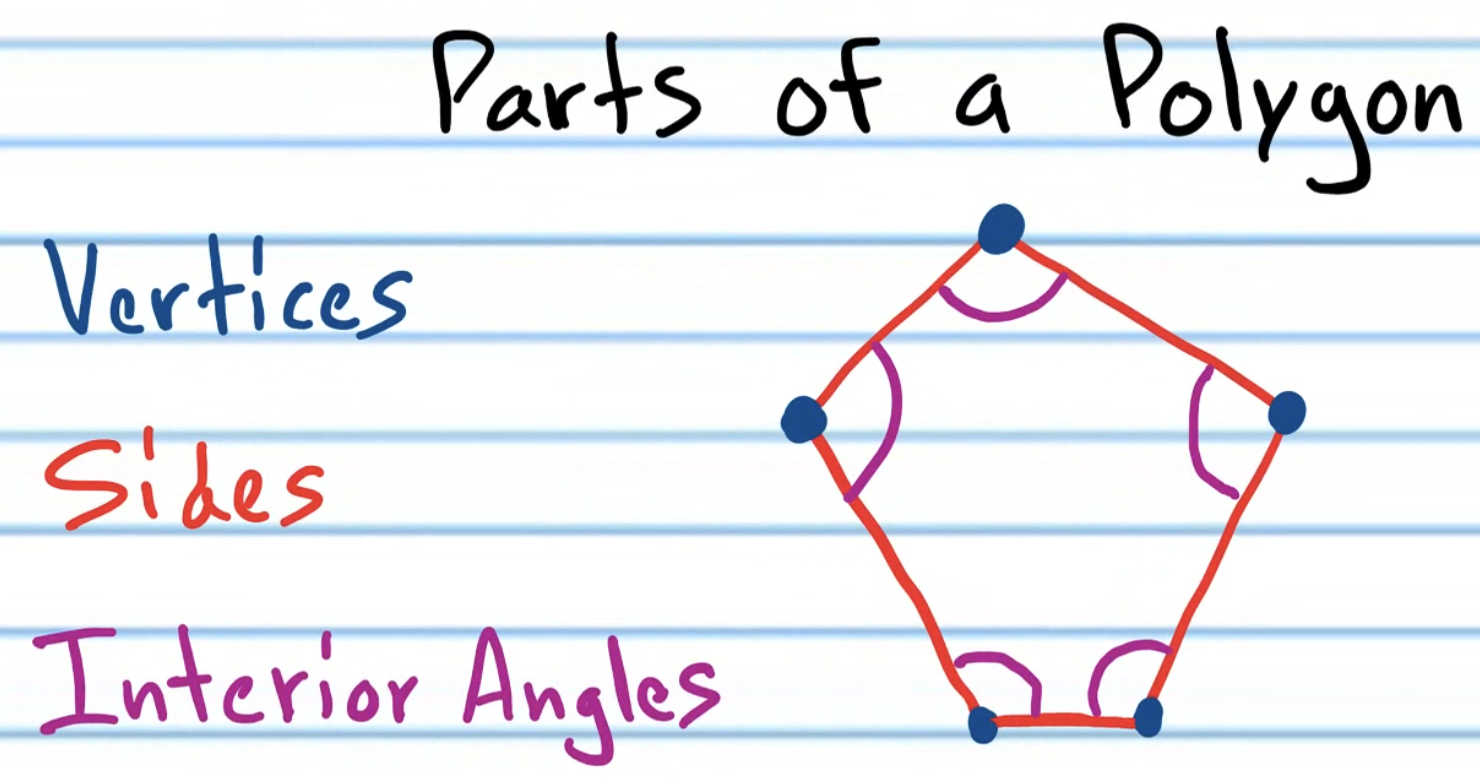
\includegraphics[width=0.7\textwidth]{0402.png}
  \caption{Parts of a Polygons}
\end{figure}

Names of Polygons

\begin{center}
\begin{tabular}{ c | c }
  \textbf{Sides} & \textbf{Name} \\
  \hline
  3 & Triangle \\
  4 & Quadrilateral, tứ giác \\
  5 & Pentagon \\
  6 & Hexagon \\
  7 & Heptaton, Septaton \\
  8 & Octagon \\
  9 & Nonagon \\
  10 & Decagon \\
  12 & Dodecagon \\
  n & n-gon \\
\end{tabular}
\end{center}

\begin{figure}[htb!]
  \centering
  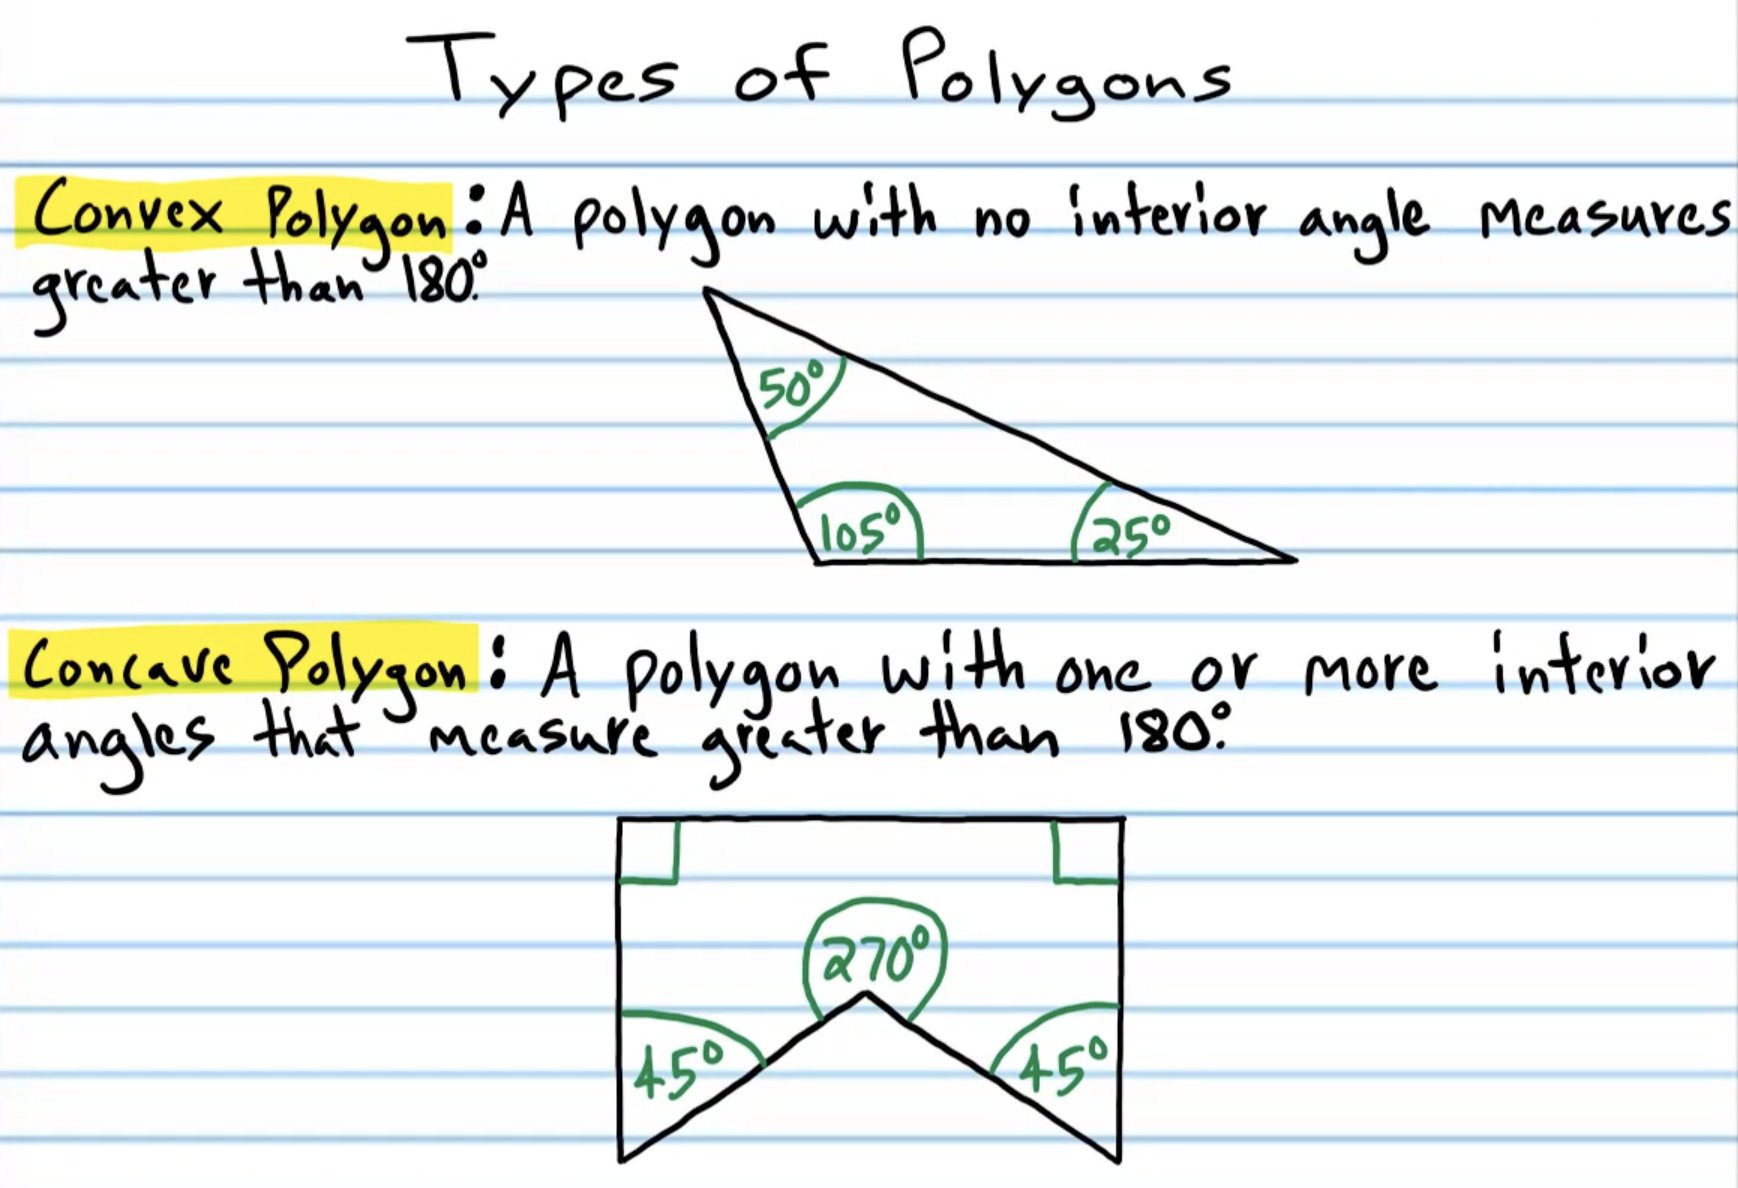
\includegraphics[width=0.8\textwidth]{0403.png}
  \caption{Types of Polygons}
\end{figure}

Convex: curving out; concave is curving in (bị lõm).

